\chapter{Activities}

In this chapter we describe the different activities that are used in our Android application. Figure~\ref{fig:activitiesLifeCycle} shows the life cycle of all our activities and provides a global view of the structure of our application. The 'Home' activity is our main activity. This is the first activity that is started when our application is launched. The user can then start further activities from this activity, such as the 'City' activity or the 'All Cities' activity. Notice that the 'City' activity can be started from the 'Home' activity but also from the 'All Cities' activity. Afterwards, the user can start from the 'City' activity the 'Mystery Tab' activity which includes the 'Mystery Map' activity and the 'Mystery Info' activity. The 'Mystery Map' activity allows the user to start different 'Challenge' activities, such as the 'Choose Date' activity, the 'Choose Picture' activity, the 'Guess Name' activity or the 'Find Direction' activity. Finally each activity, except of the individual challenge activities, has access to a menu which includes the 'Settings' activity, 'Help' activity and the 'About' activity.

\begin{figure}[H]
	\centering
	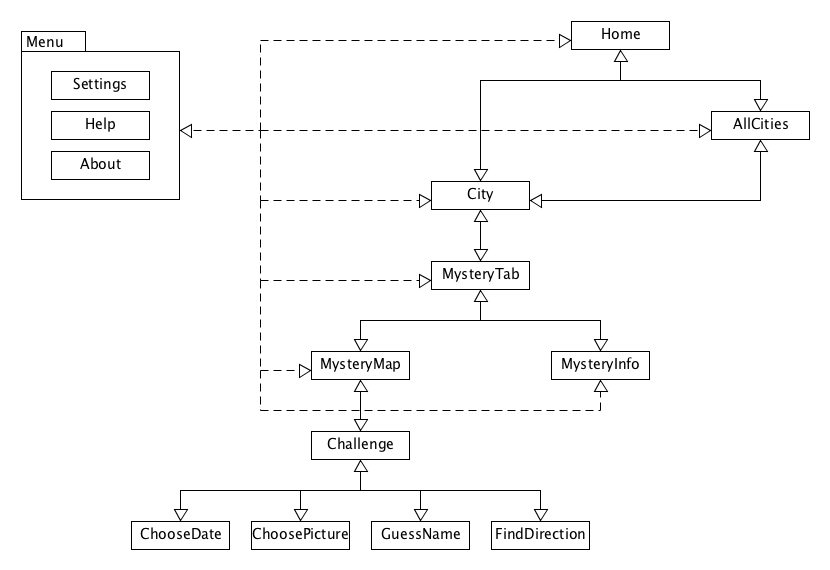
\includegraphics[scale=0.4]{Figures/ActivityLifeCycle}
	\caption{Life cycle of all activities.}
	\label{fig:activitiesLifeCycle}
\end{figure}

\section{Home Activity}

The 'Home' activity is our main activity. This is the first activity that the user sees and that is started at the launch of our application. It loads the JSON persistent data and creates the necessary data structure. It also displays the total score that the user has achieved so far. It provides an 'All Cities' button, which allows a user to start the 'All Cities' activity. However, based on the user's current location it also able to suggest to the user the closest city near by.

\begin{figure}[H]
	\centering
	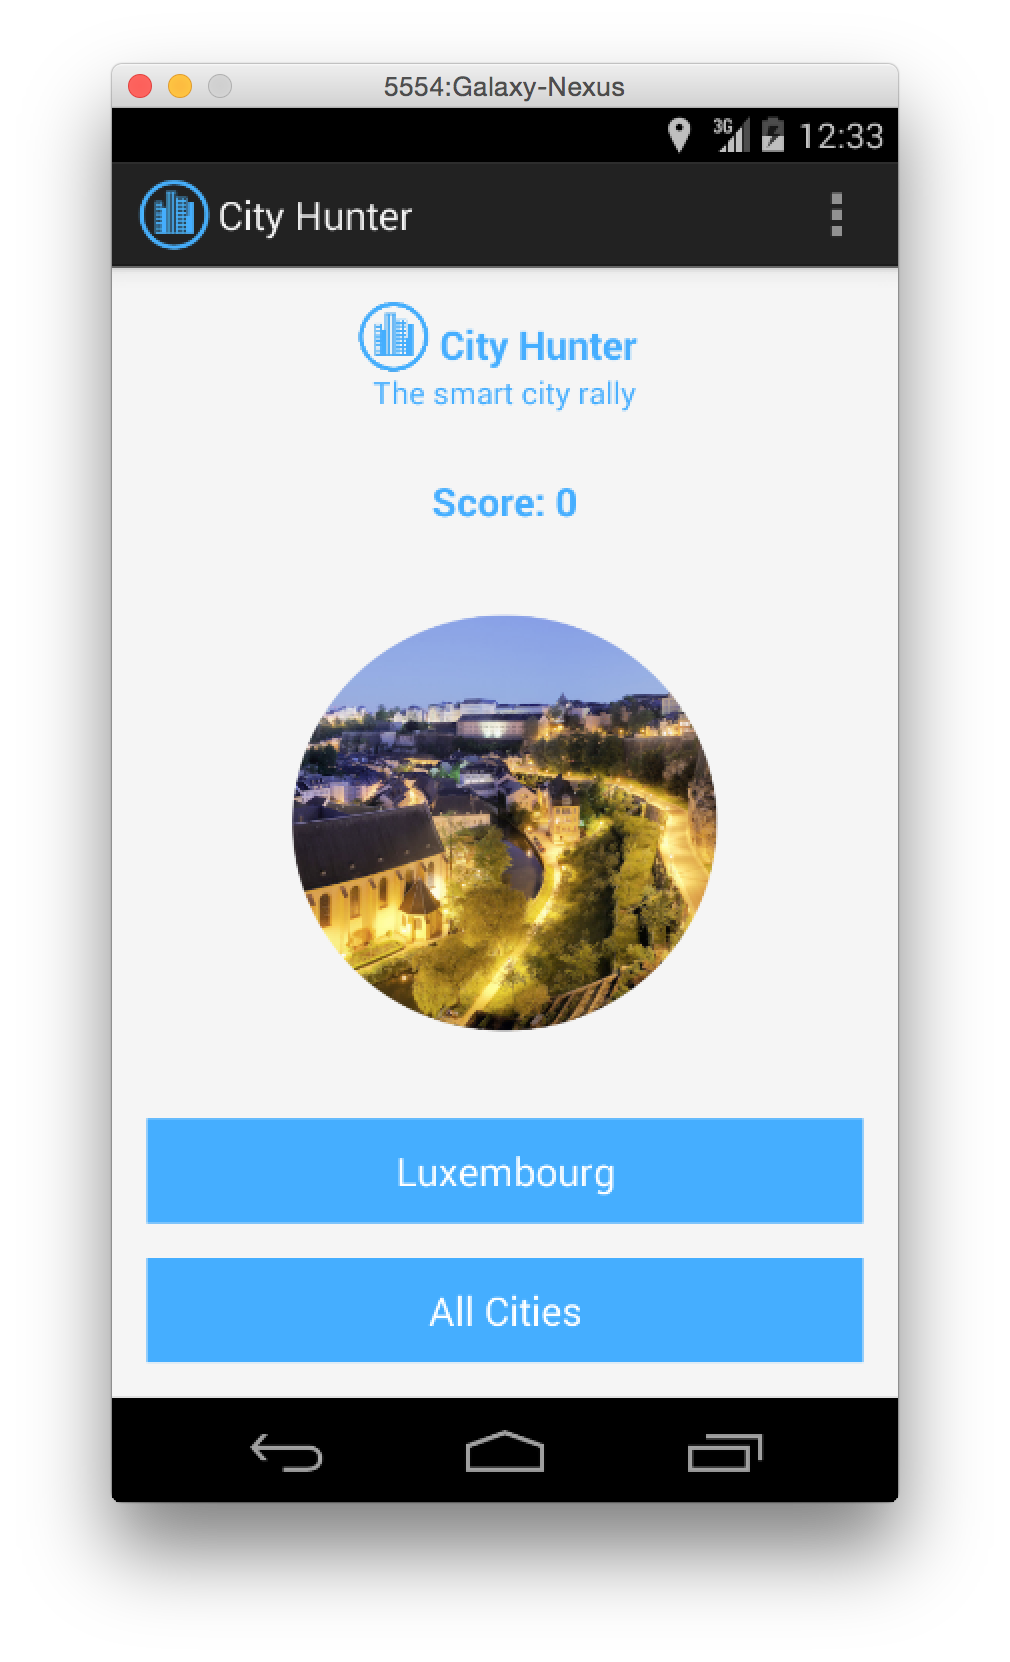
\includegraphics[scale=0.4]{Figures/HomeActivity}
	\caption{A snapshot of the Home Activity.}
\end{figure}

\section{All Cities Activity}

The 'All Cities' activity shows all available cities in a grid list. The user can select an individual city out of this list to start the 'City' activity which displays more details about the selected city.

\begin{figure}[H]
	\centering
	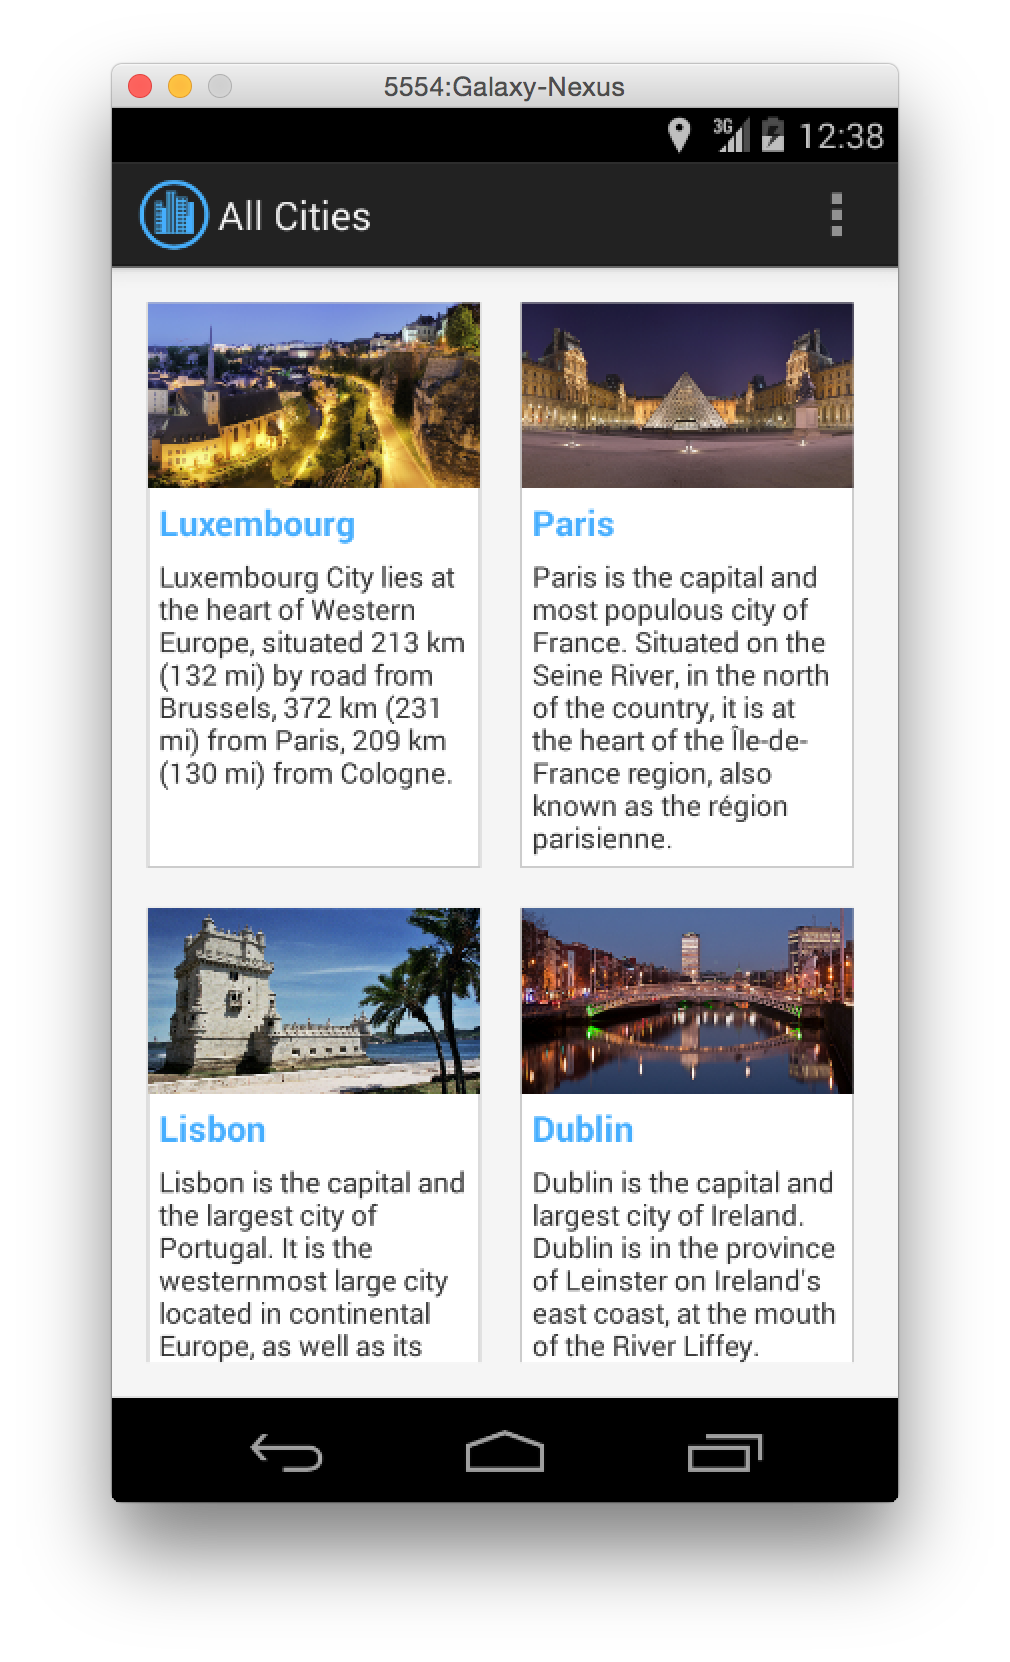
\includegraphics[scale=0.4]{Figures/AllCitiesActivity}
	\caption{A snapshot of the All Cities Activity.}
\end{figure}

\section{City Activity}

The 'City' activity shows all available mysteries for a particular city in a grid list. The user can select an individual mystery out of this list to start the 'Mystery Tab' activity.

\begin{figure}[H]
	\centering
	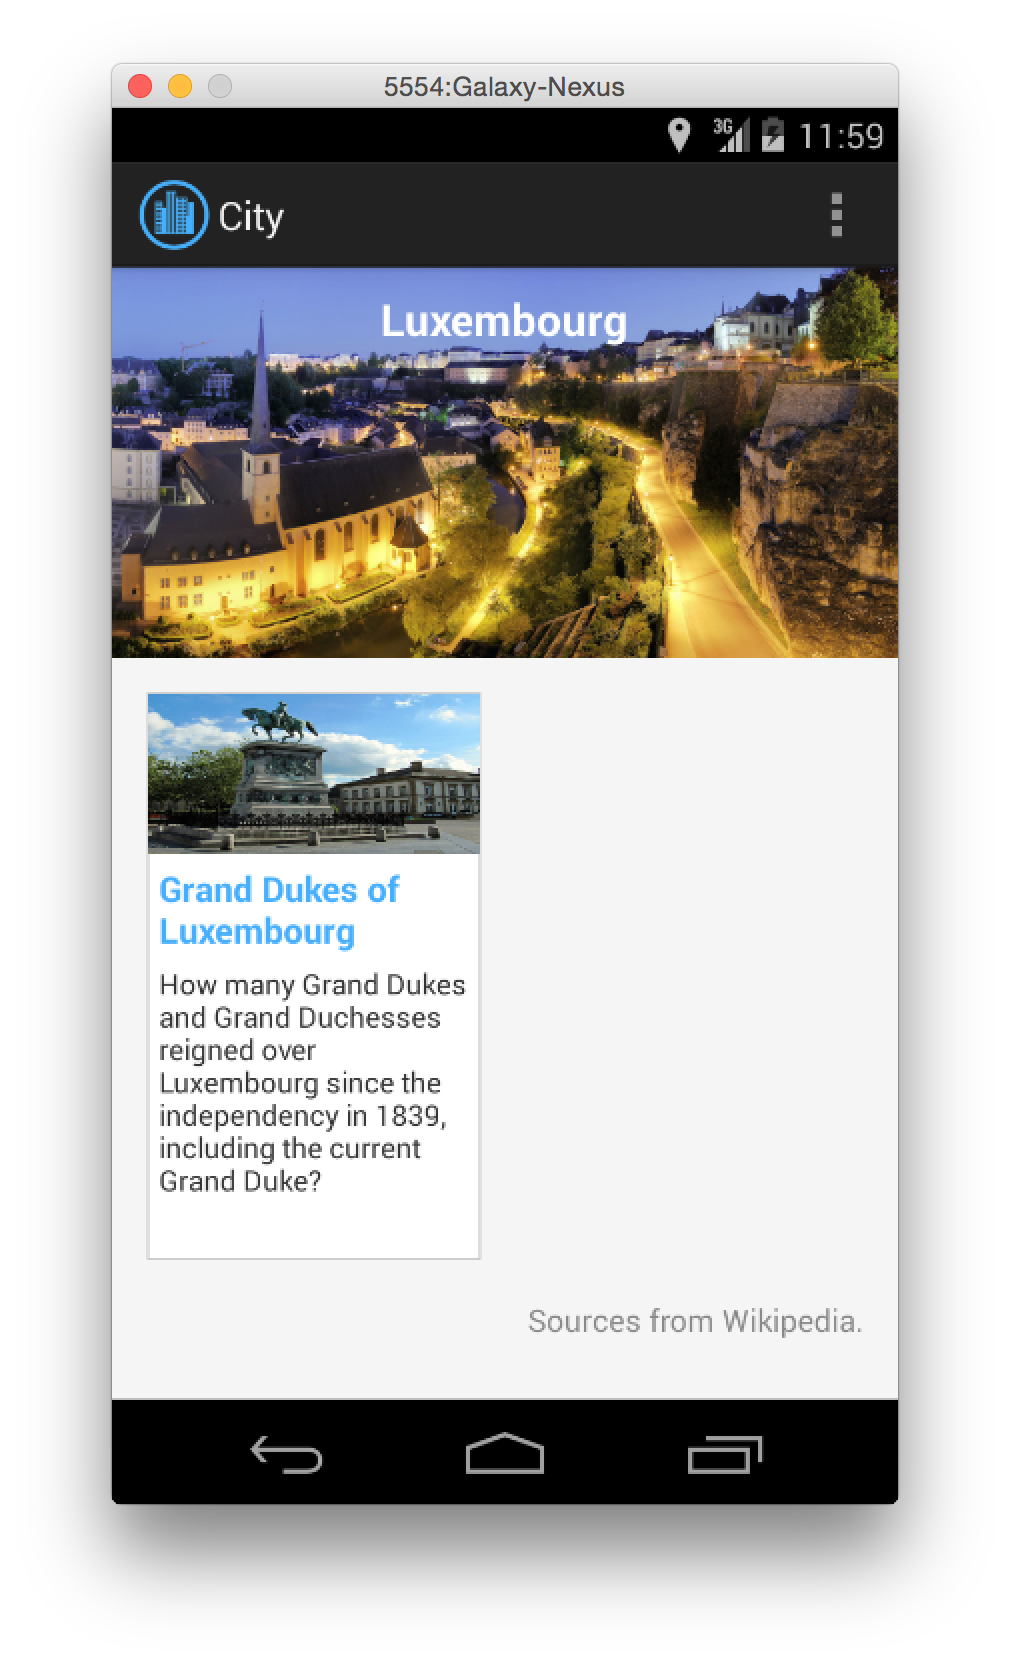
\includegraphics[scale=0.4]{Figures/CityActivity}
	\caption{A snapshot of the City Activity.}
\end{figure}

\section{Mystery Map Activity}

The 'Mystery Map' activity is the first tab of the 'Mystery Tab' activity. It shows a map with all the available challenges. The map also contains a button to switch to fullscreen and a button to route the user from his current location to the closest challenge. Below the map is a list of all available challenges. Challenges are normally inactive and only become active if the user's current position is close to a challenge. Each inactive challenge has a button which when pressed shows the route from the user's current location to the particular challenge. Active challenges can be clicked on to start the particular 'Challenge' activity.

\begin{figure}[H]
	\centering
	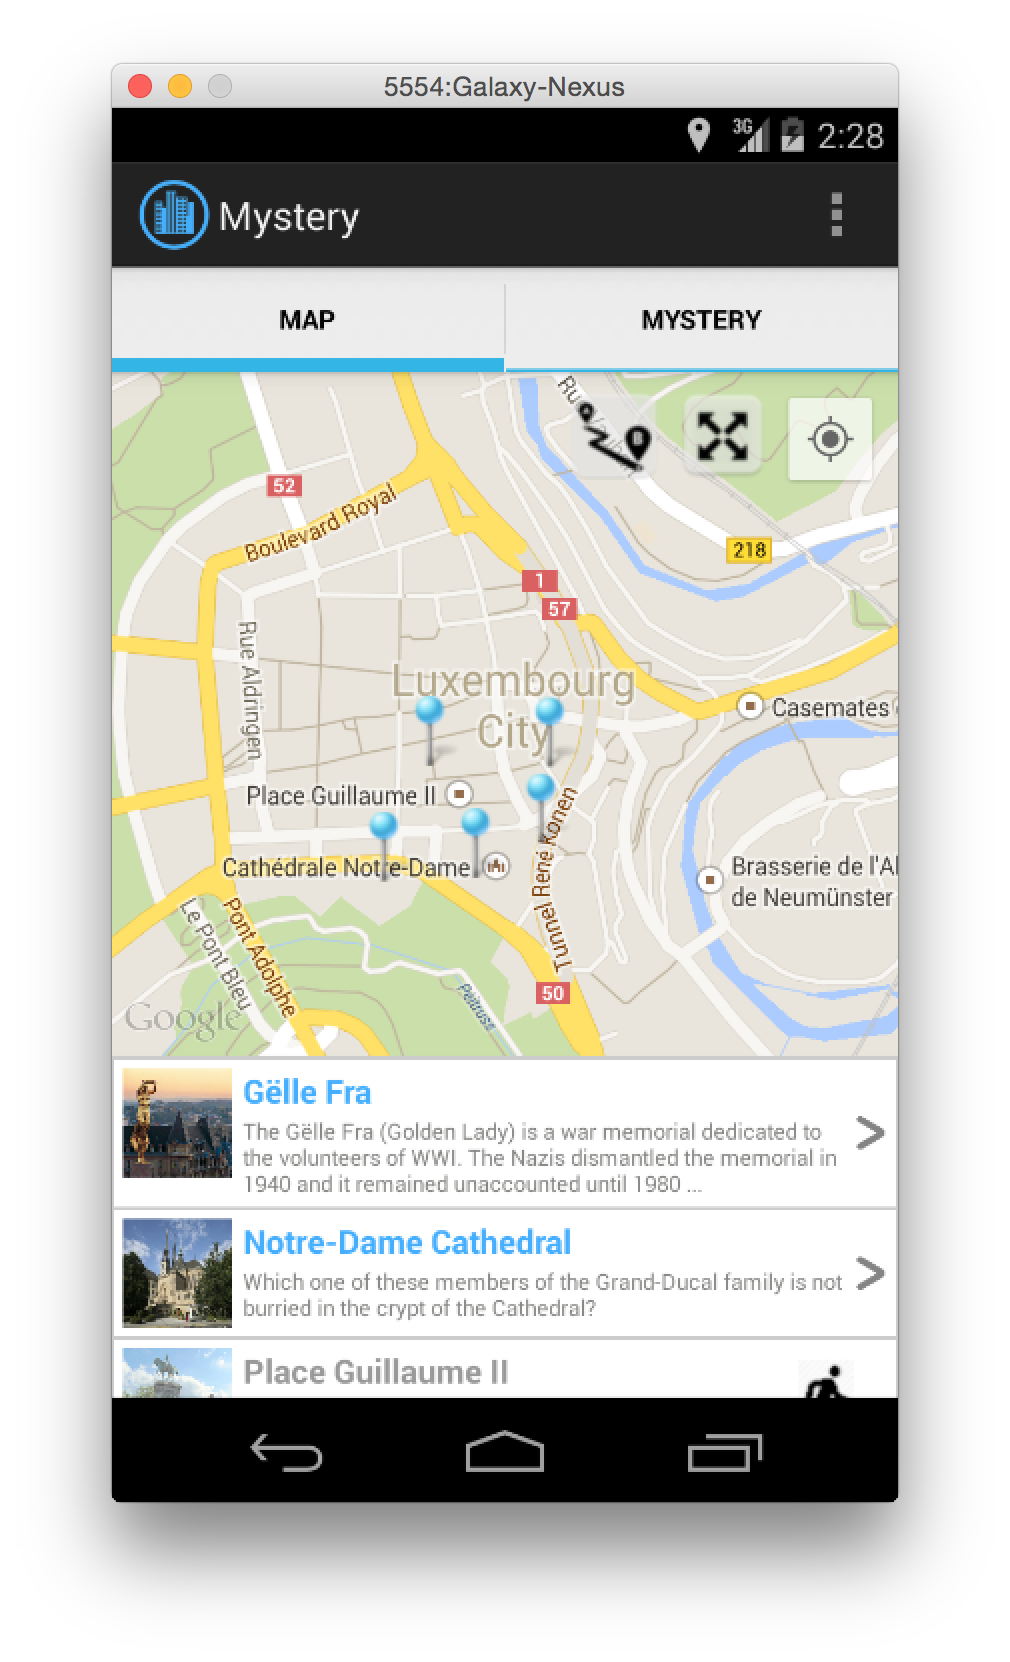
\includegraphics[scale=0.4]{Figures/MysteryMapActivity}
	\caption{A snapshot of the Mystery Map Activity.}
\end{figure}

\section{Mystery Info Activity}

The 'Mystery Info' activity is the second tab of the 'Mystery Tab' activity. It shows the title and the question of the mystery that the user has to solve. If the user was able to successfully complete all the challenges, then also a hint is displayed to help the user solving the mystery. Finally, the activity also provides to the user a way to enter his answer for the mystery.

\begin{figure}[H]
	\centering
	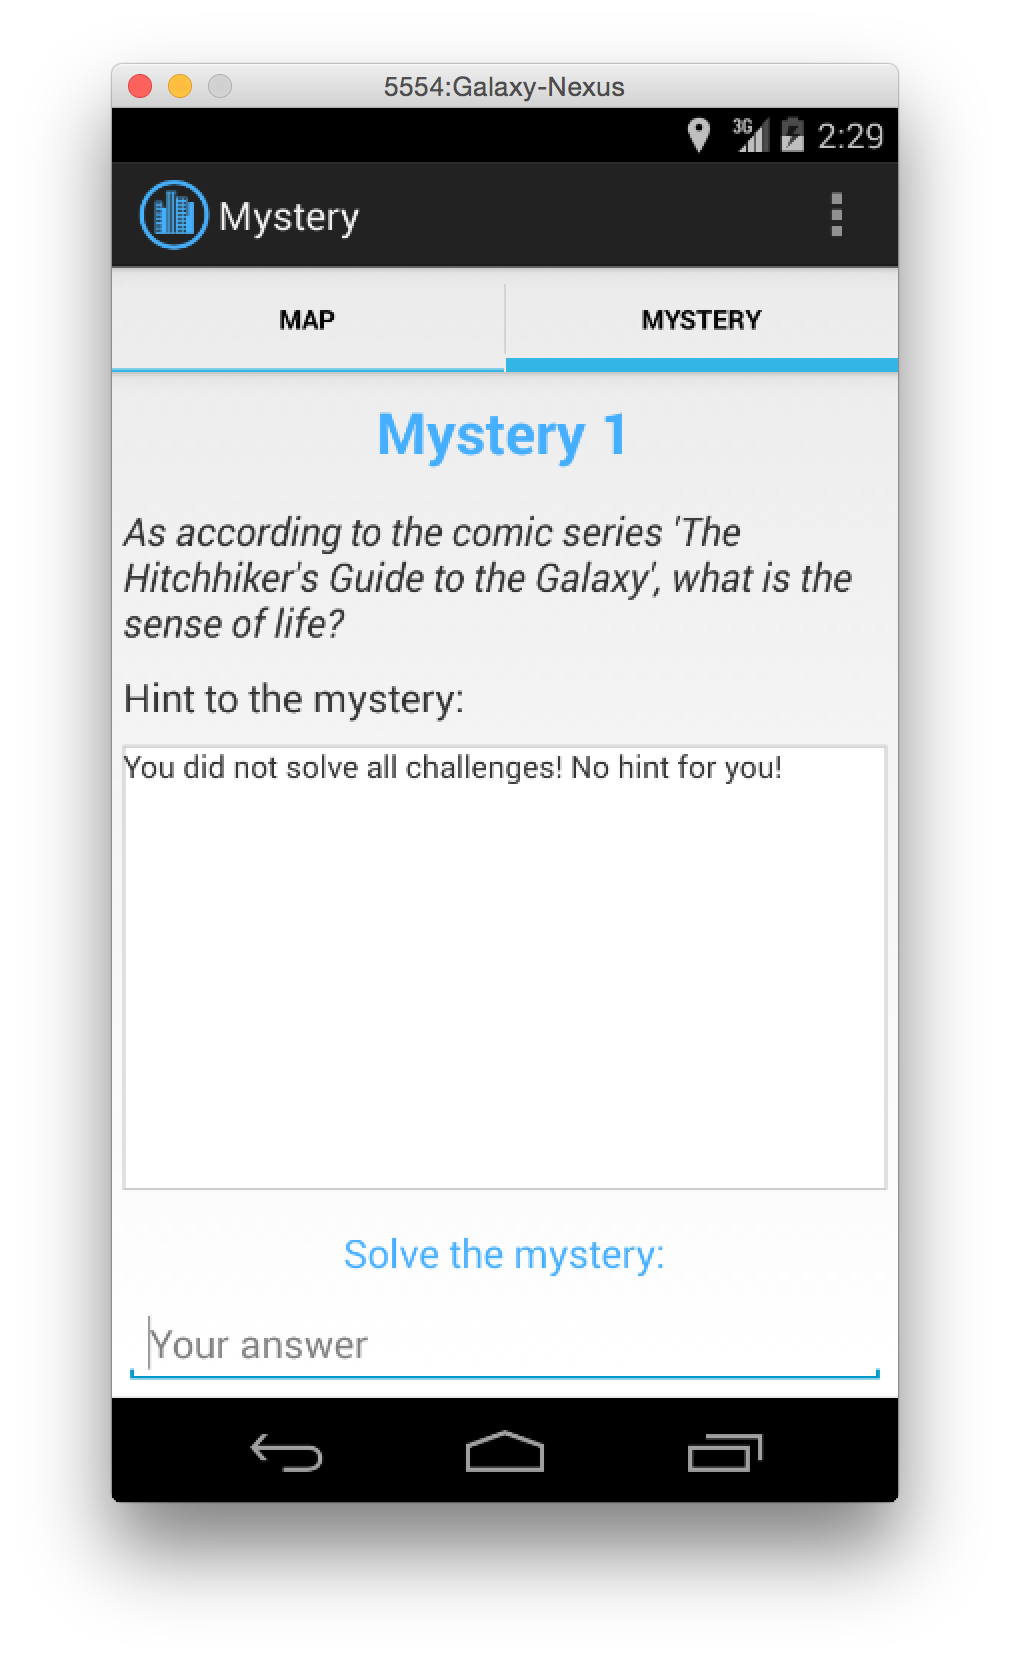
\includegraphics[scale=0.4]{Figures/MysteryInfoActivity}
	\caption{A snapshot of the Mystery Info Activity.}
\end{figure}

\section{Challenge Activity}

The 'Challenge' activity loads individual challenge activities relative to the selected type of challenge in the 'Mystery Map' activity. Possible challenge activities are: 

\begin{itemize}
	\item Choose Date Activity
	\item Choose Picture Activity
	\item Guess Name Activity
	\item Find Direction Activity
\end{itemize}

\begin{figure}[H]
	\centering
	\begin{subfigure}[b]{0.3\textwidth}
                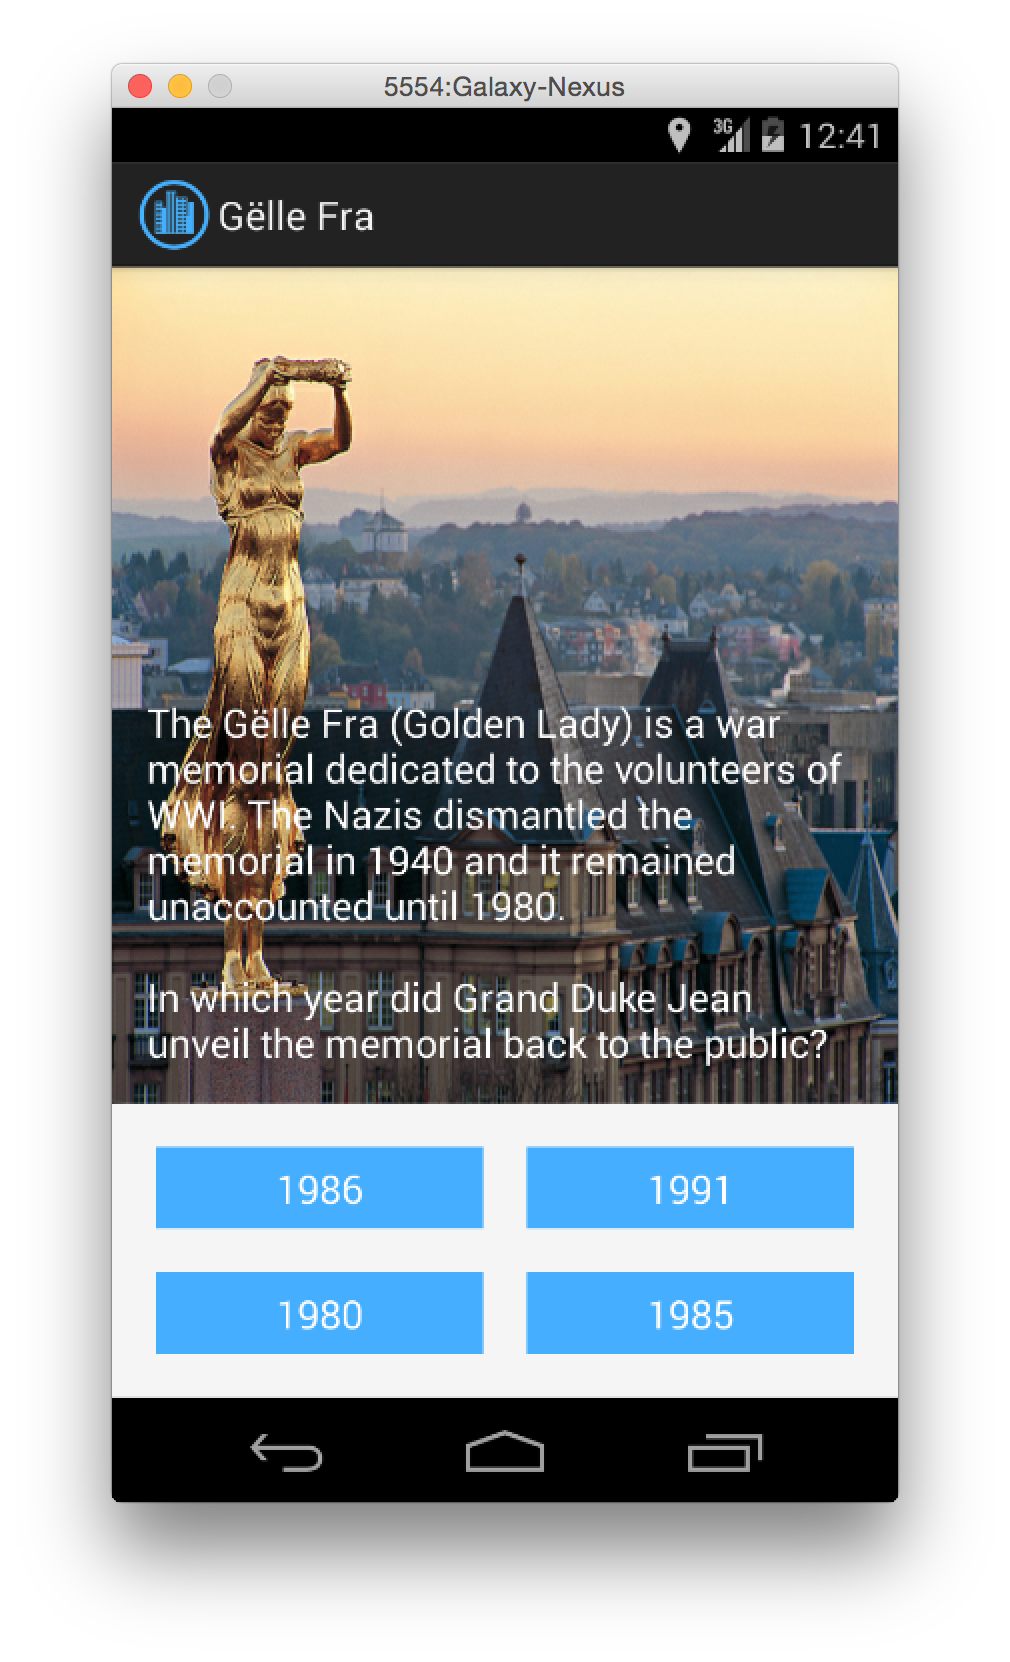
\includegraphics[width=\textwidth]{Figures/ChooseDateActivity}
                \caption{Choose Date Activity}
        \end{subfigure}%
	\begin{subfigure}[b]{0.3\textwidth}
                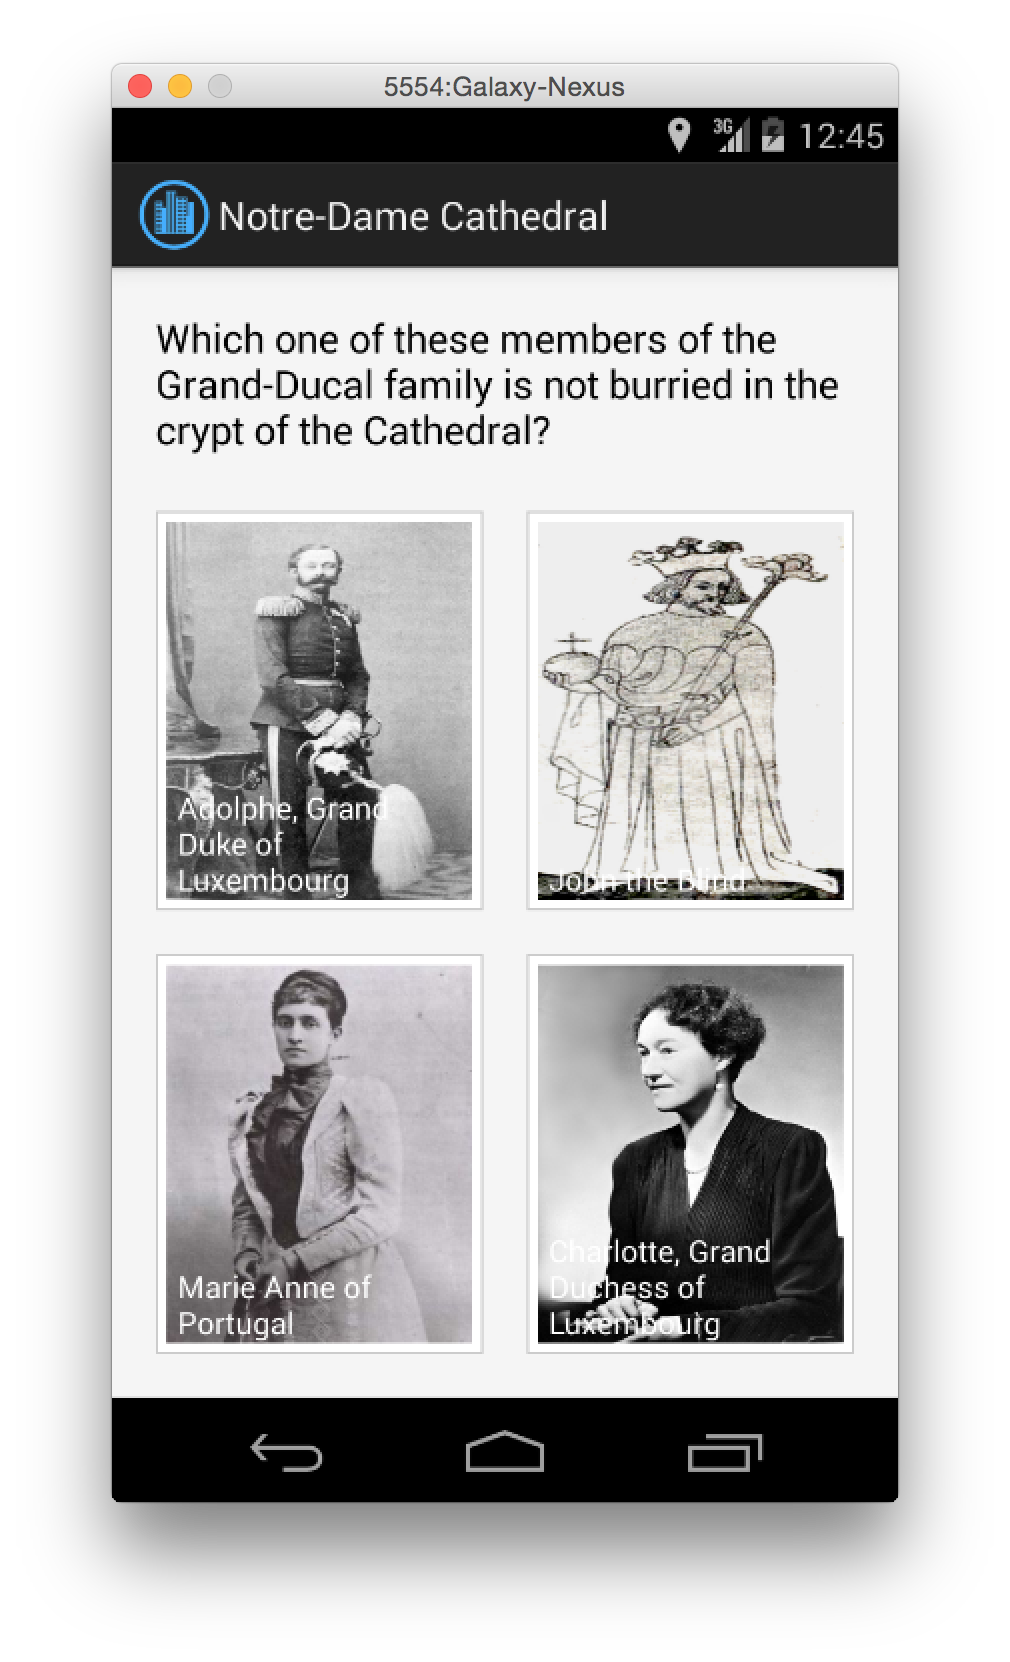
\includegraphics[width=\textwidth]{Figures/ChoosePictureActivity}
                \caption{Choose Picture Activity}
        \end{subfigure}
	\begin{subfigure}[b]{0.3\textwidth}
                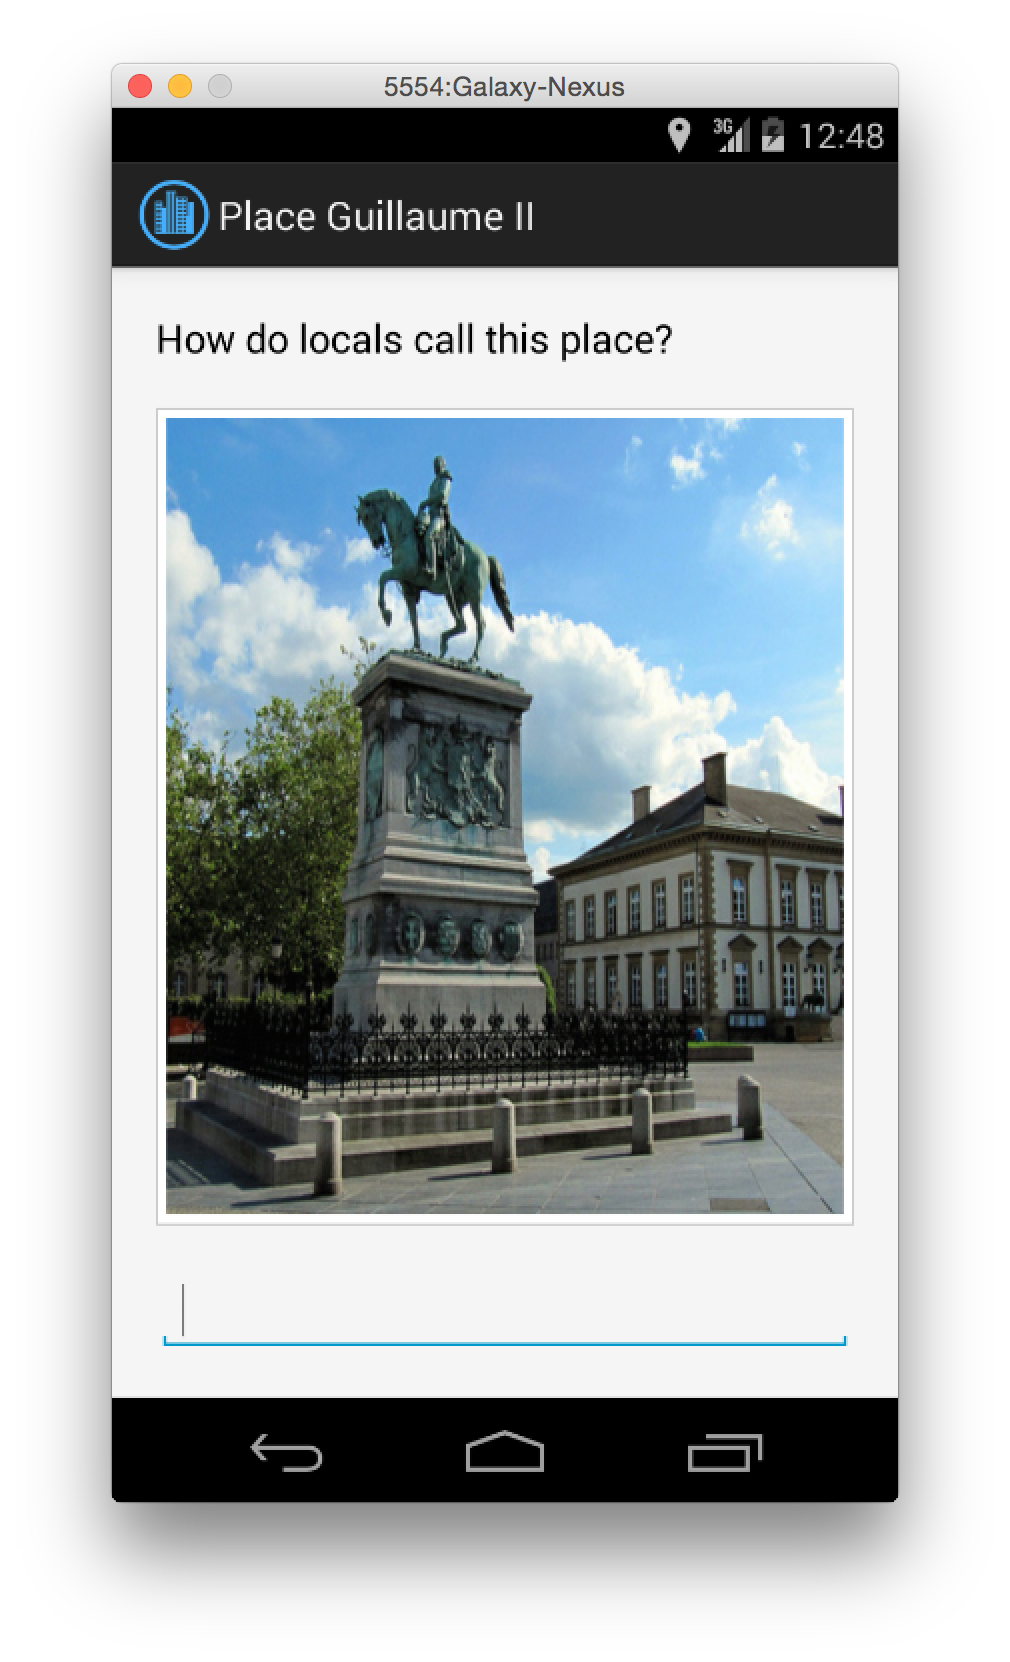
\includegraphics[width=\textwidth]{Figures/GuessNameActivity}
                \caption{Guess Name Activity}
        \end{subfigure}%
	\begin{subfigure}[b]{0.3\textwidth}
                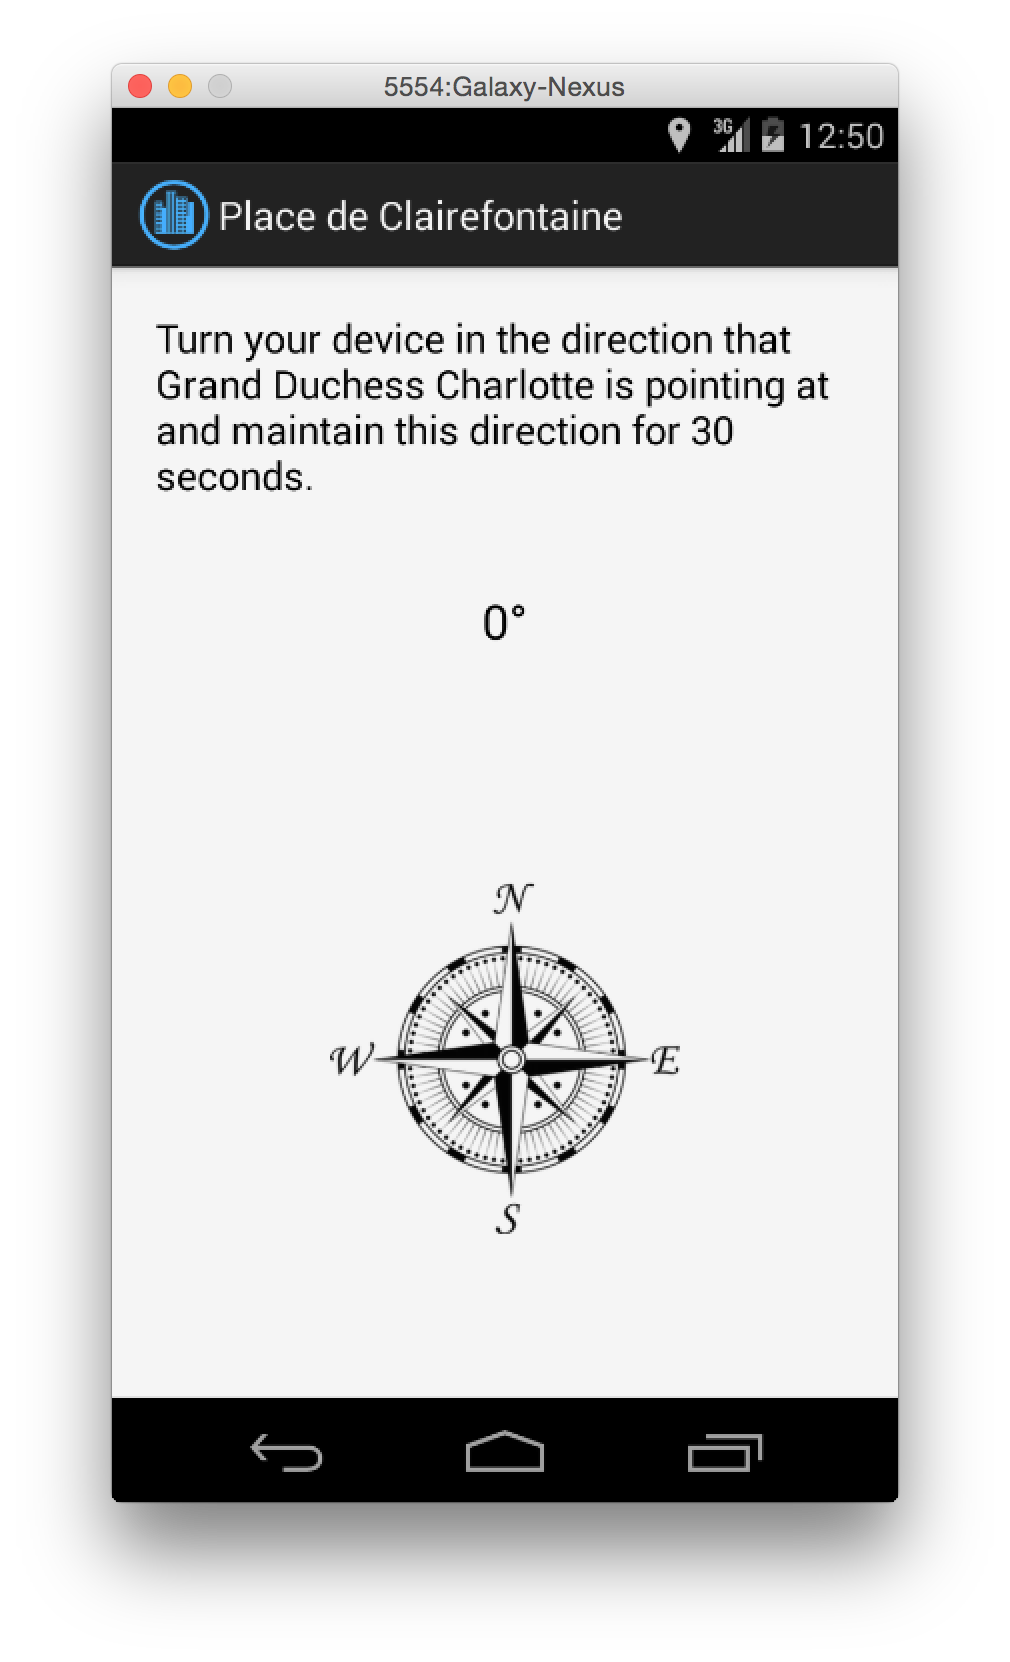
\includegraphics[width=\textwidth]{Figures/FindDirectionActivity}
                \caption{Find Direction Activity}
        \end{subfigure}
        \caption{Snapshots of the possible challenge activities.}
\end{figure}

\section{Menu Activity}

Each activity, except of the challenge activities, has access to a menu which provides a selection of the following three activities: 

\begin{itemize}
	\item Settings Activity
	\item Help Activity
	\item About Activity
\end{itemize}

\noindent
The 'Settings' activity provides a button to reset all saved data, including the user's progress and his current score. The 'Help' activity provides a description of the application in order to help the user better understand how the application works. The 'About' activity includes a small description and information about the copyright and the authors of the application.

\begin{figure}[H]
	\centering
	\begin{subfigure}[b]{0.3\textwidth}
                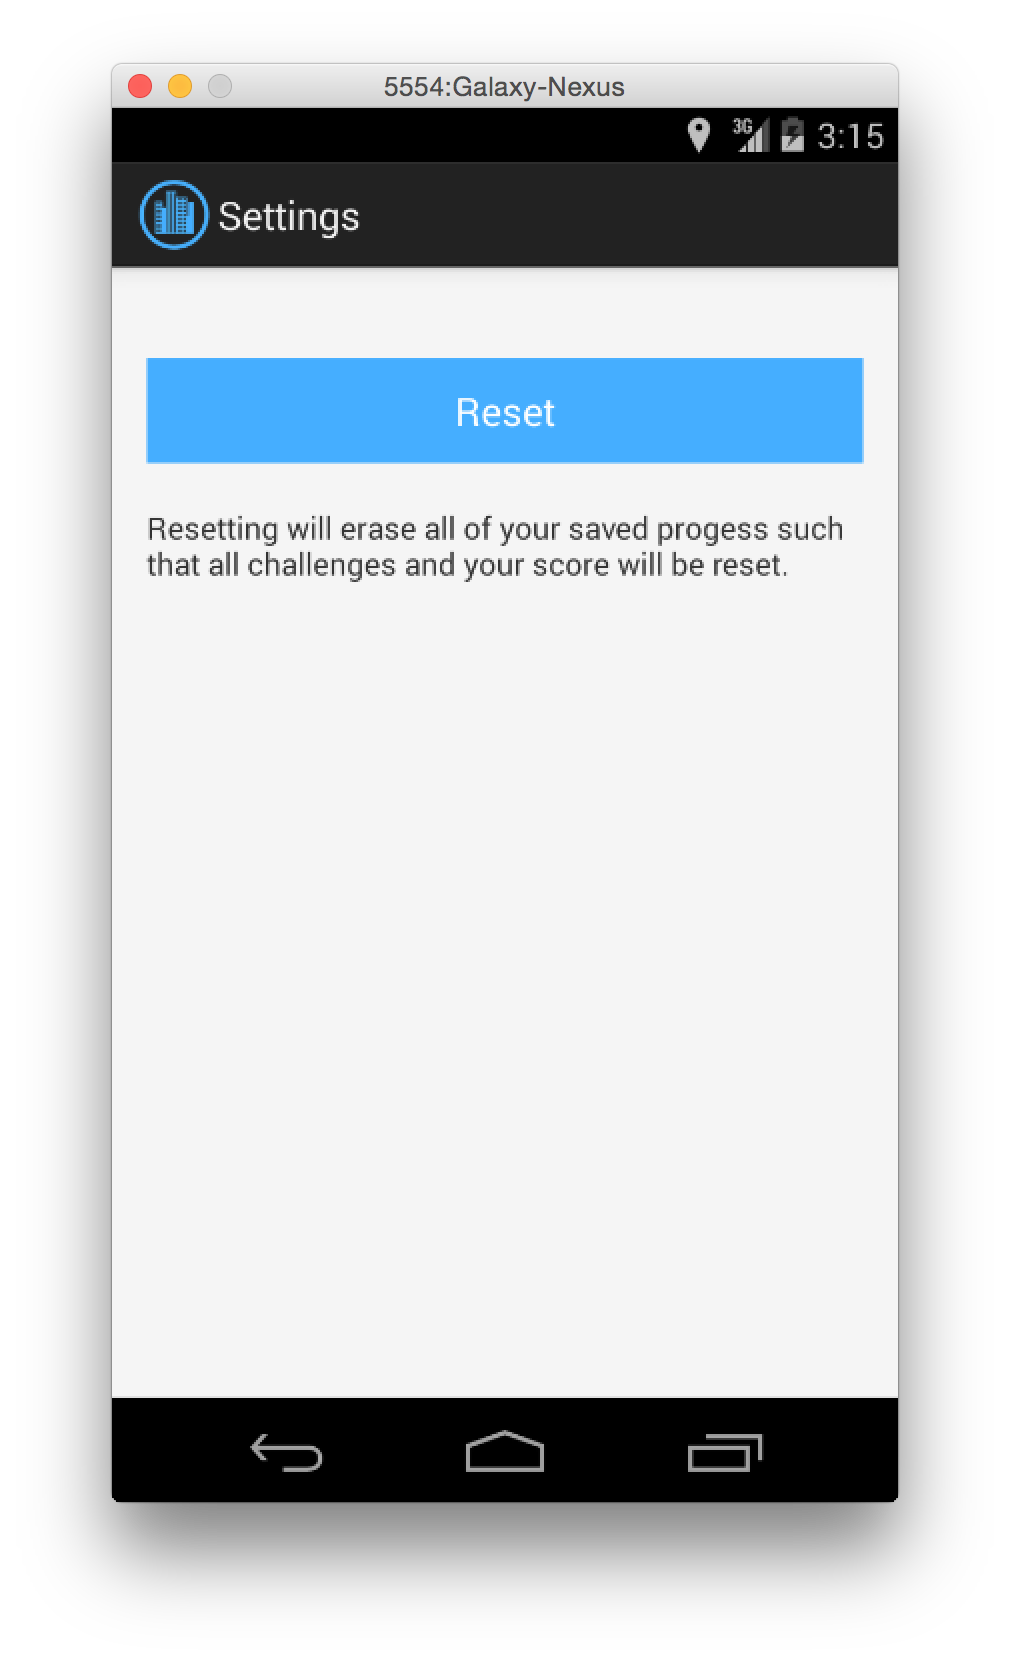
\includegraphics[width=\textwidth]{Figures/SettingsActivity}
                \caption{Settings Activity}
        \end{subfigure}
	\begin{subfigure}[b]{0.3\textwidth}
                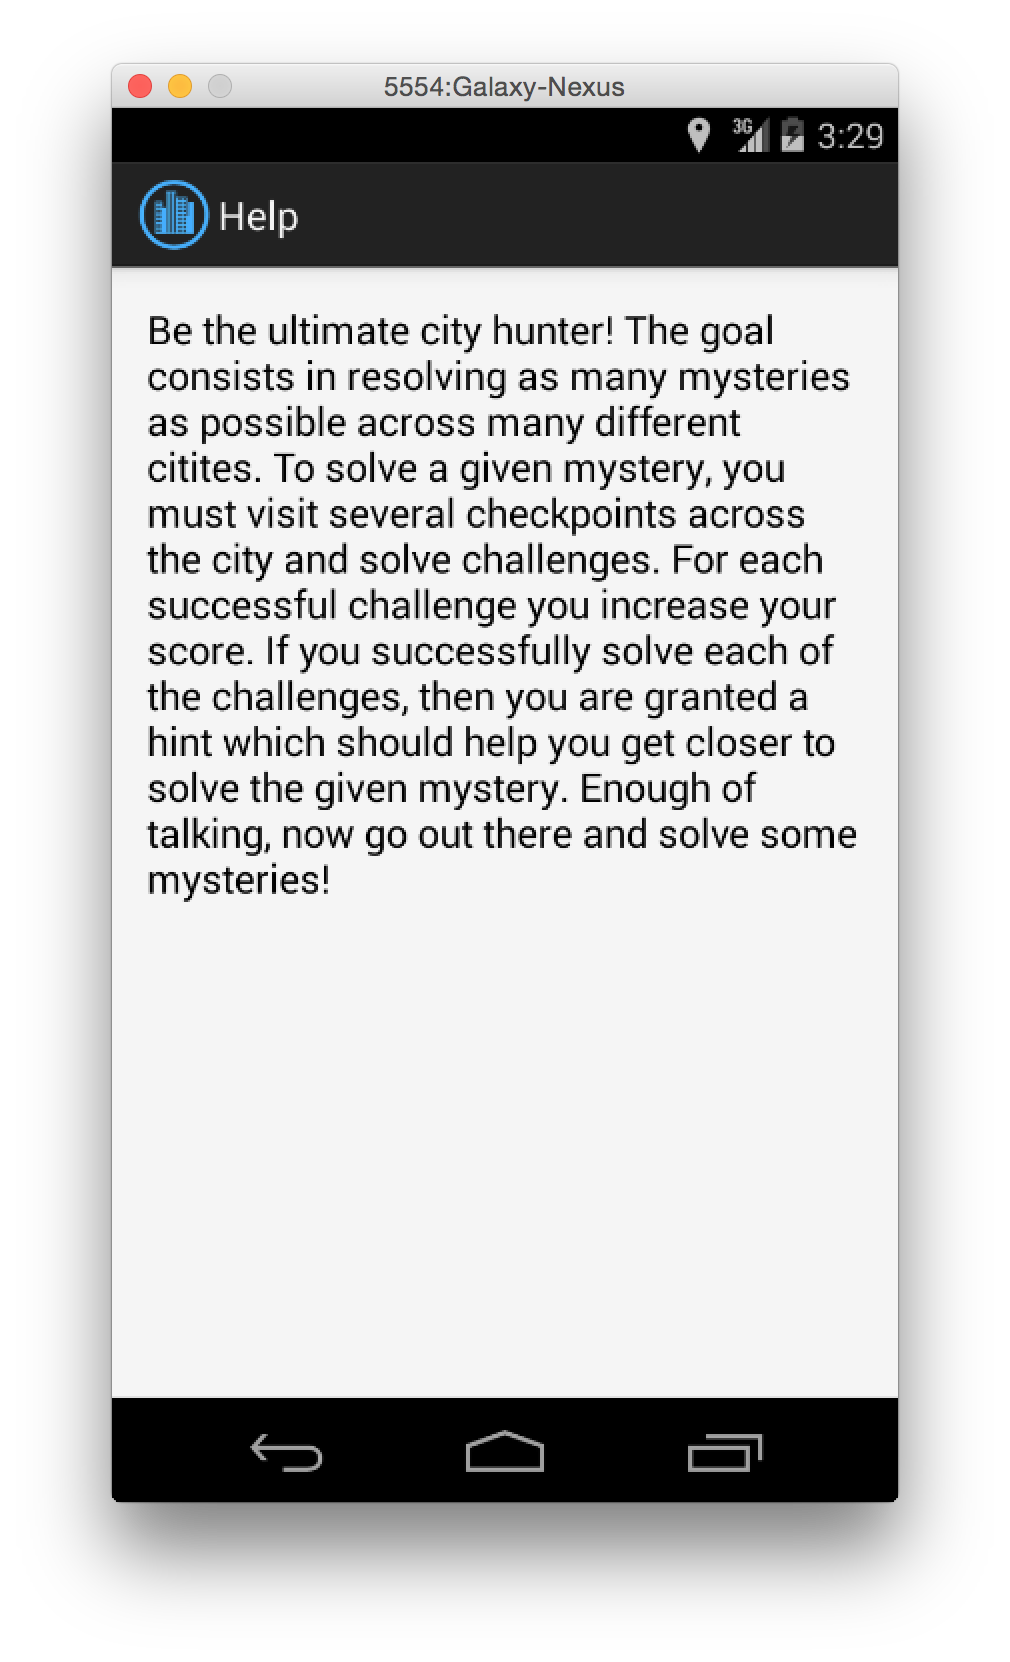
\includegraphics[width=\textwidth]{Figures/HelpActivity}
                \caption{Help Activity}
        \end{subfigure}
	\begin{subfigure}[b]{0.3\textwidth}
                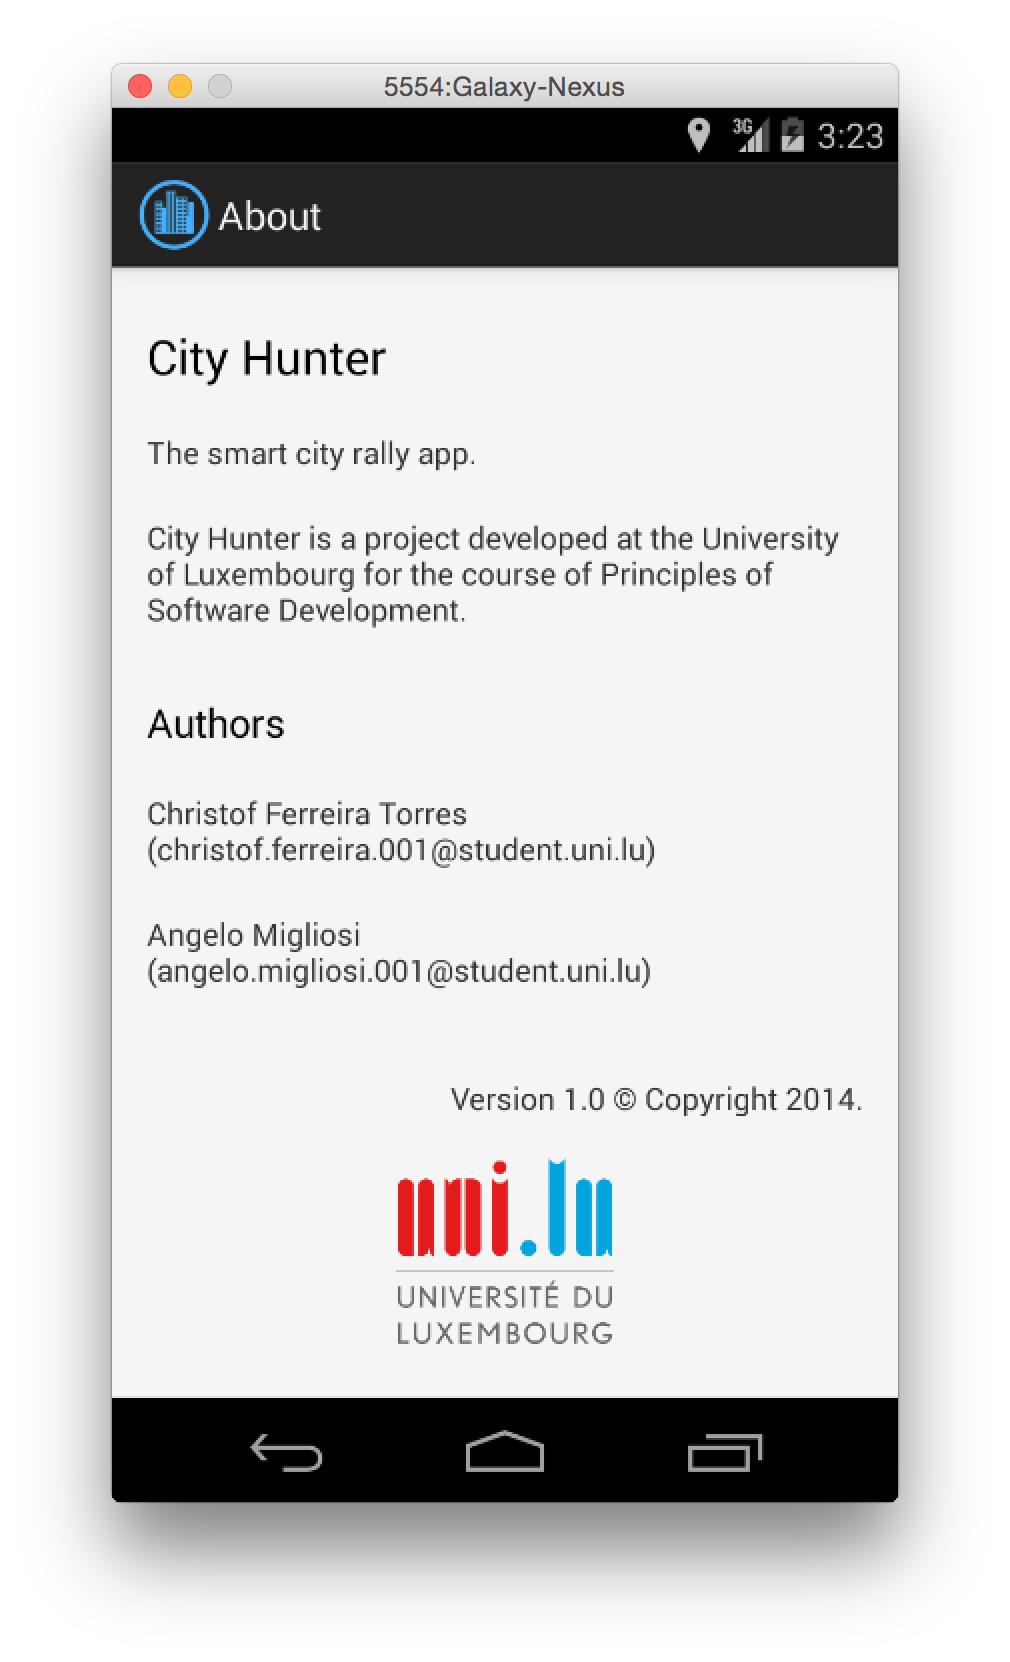
\includegraphics[width=\textwidth]{Figures/AboutActivity}
                \caption{About Activity}
        \end{subfigure}
        \caption{Snapshots of the three menu activities.}
\end{figure}
